\chapter{Experimental Approach (10 pgs)}

There are many ways how to perform production of quantum turbulence (QT): by an oscillating objects (wire, the tuning fork, the torsionally oscillating disc, etc.) or by a \textit{coflow} or \textit{counterflow} techniques.

To form the QT we used the tuning fork resonator, drived by alternating source Agilent A33220 and SR830 amplifying lock-in. Signal detection was made using second sound sensors and monitored by LabView software.

All the measurements were performed in a helium cryostat, cooled down to the desired temperatures using a rotary and Roots pump, and stabilized (with errors of a few mK) either manually or using the temperature controller. Thw working temperatures are from a wide range from a little above $T_{\lambda}$ to the lowest (experimentally) possible one $T_{min} \approx 1.26\unit{K}$.

\section{Apparatus}
\begin{itemize}
	\item cryostat
	\item cooling system
	\item insert
	\item resonator
\end{itemize}

Paťova bakalárka

Apparatus:

\begin{figure}[h]
	\centering
	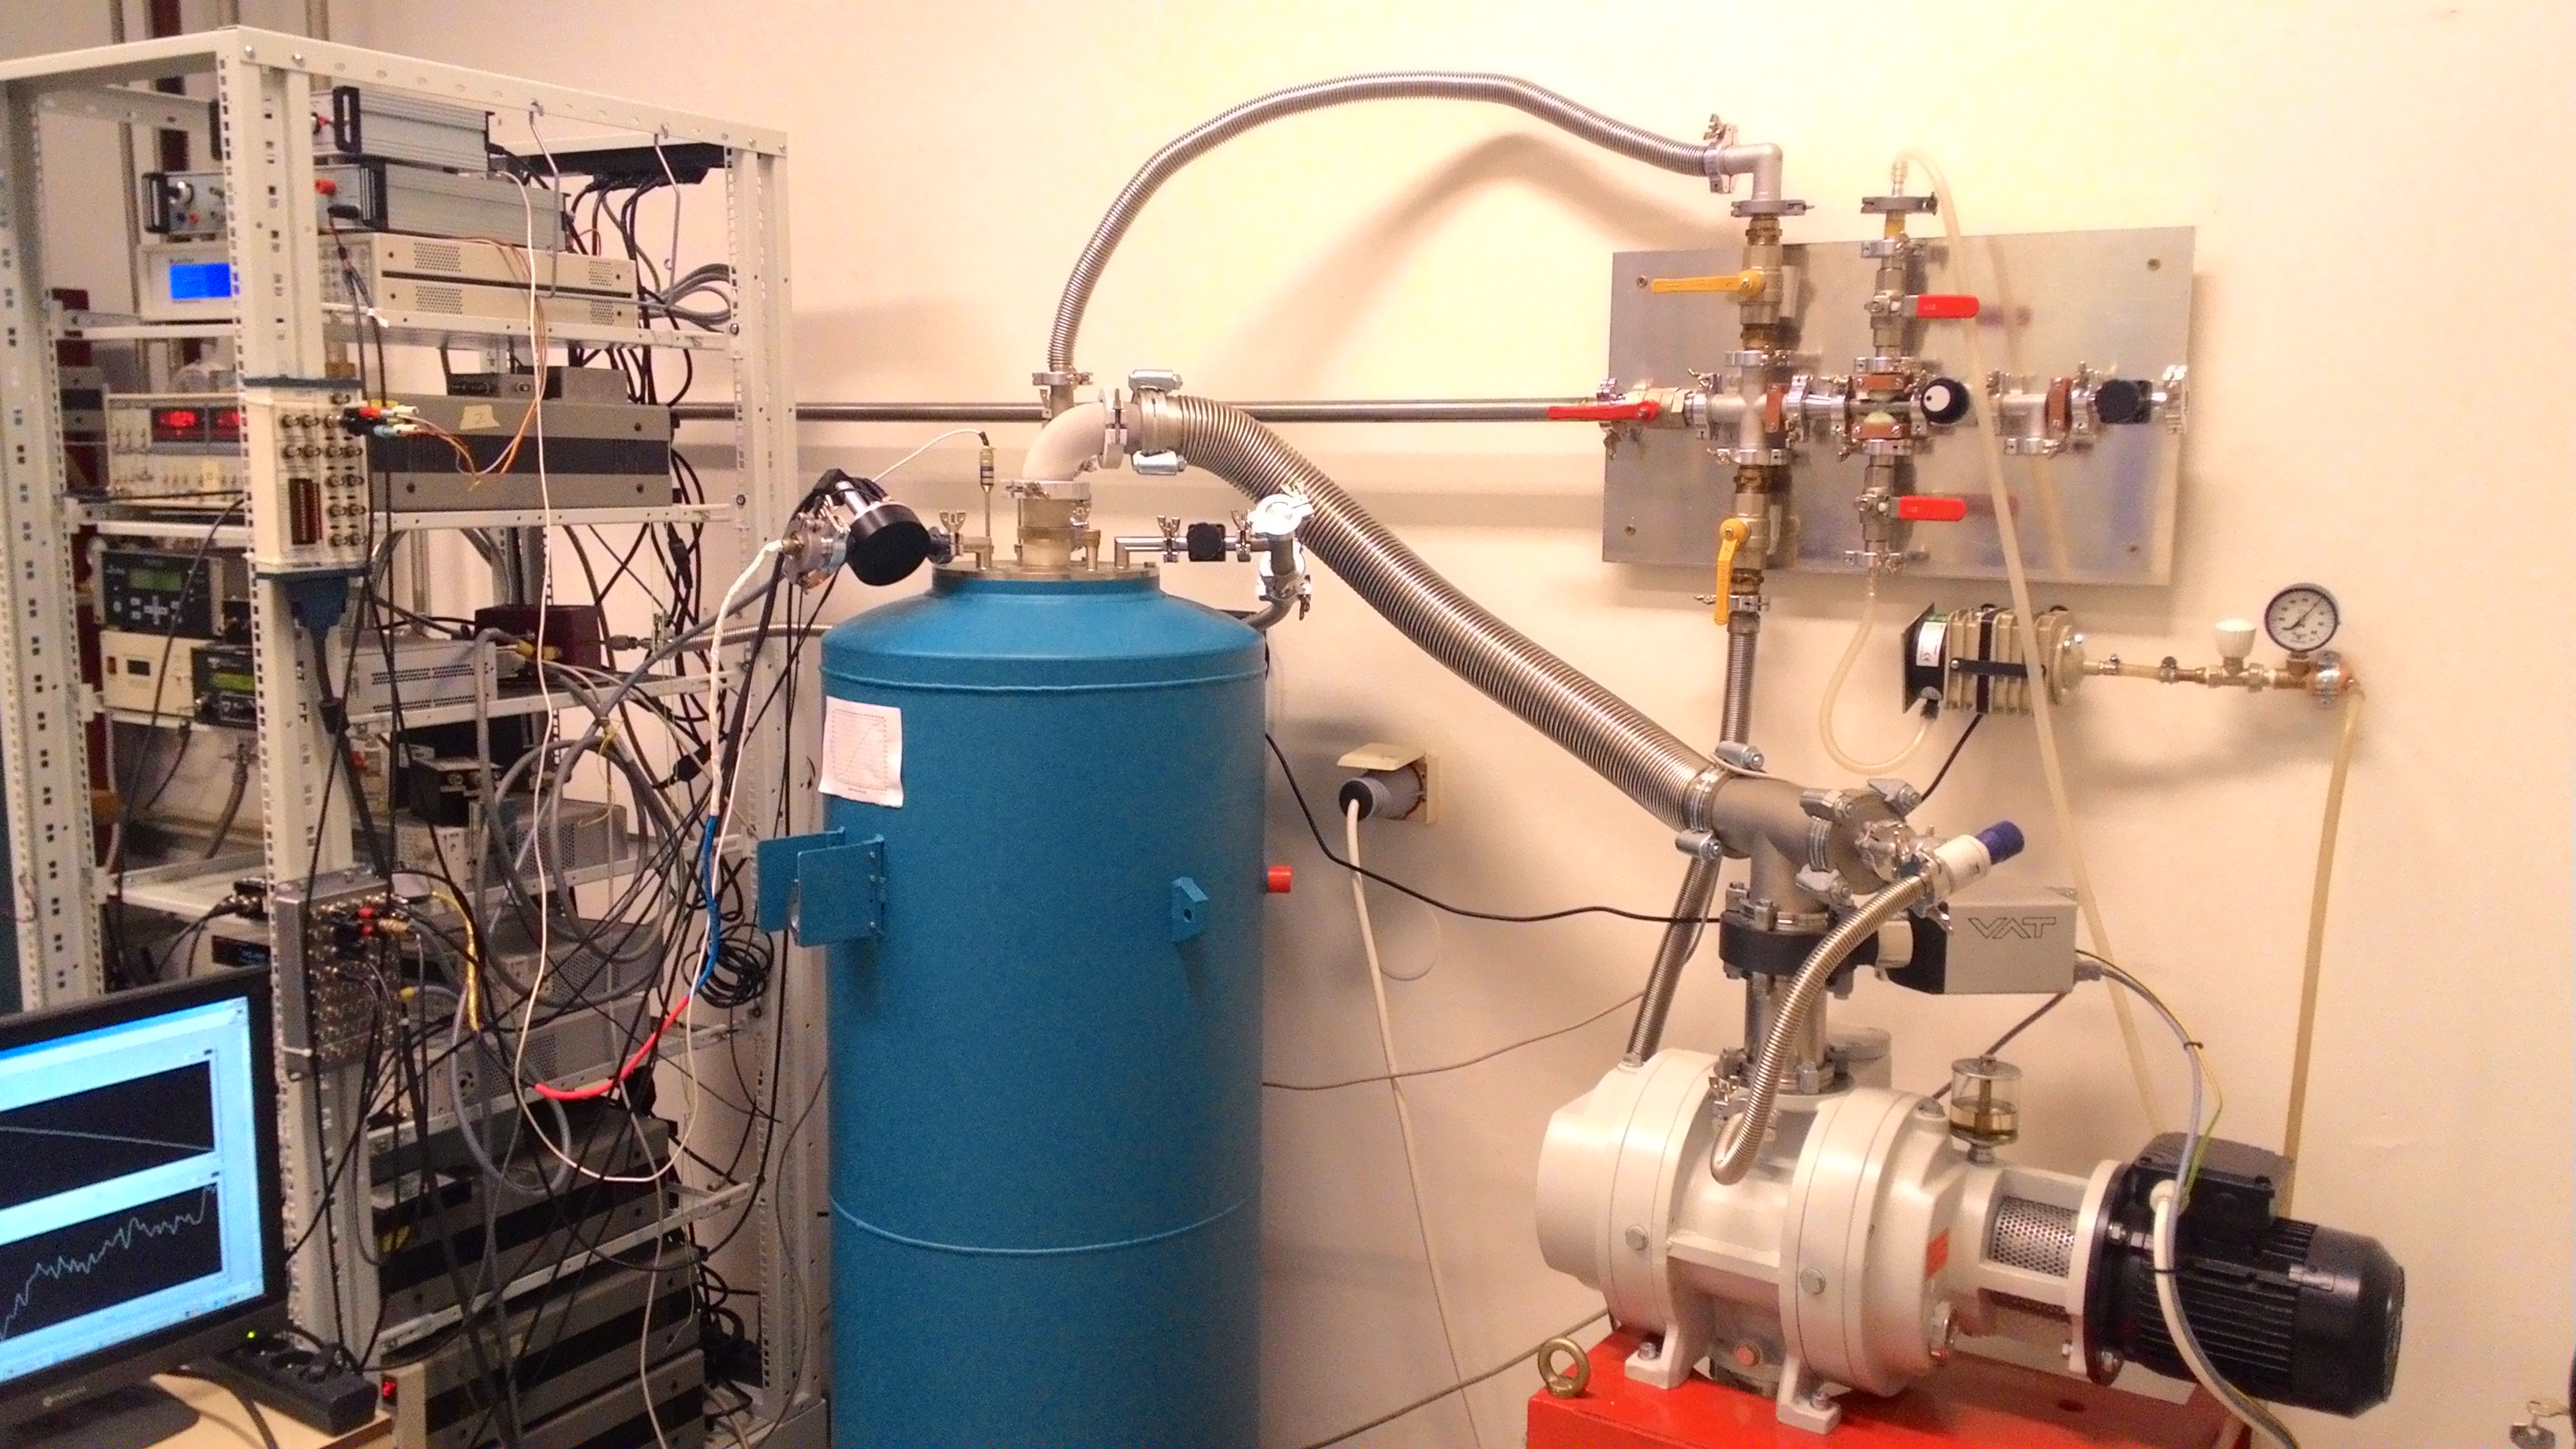
\includegraphics[width=0.5\textwidth]{graphics/exp/apparatus}
	\caption{abcd}
\end{figure}

Insert:

\begin{figure}[h]
	\centering
	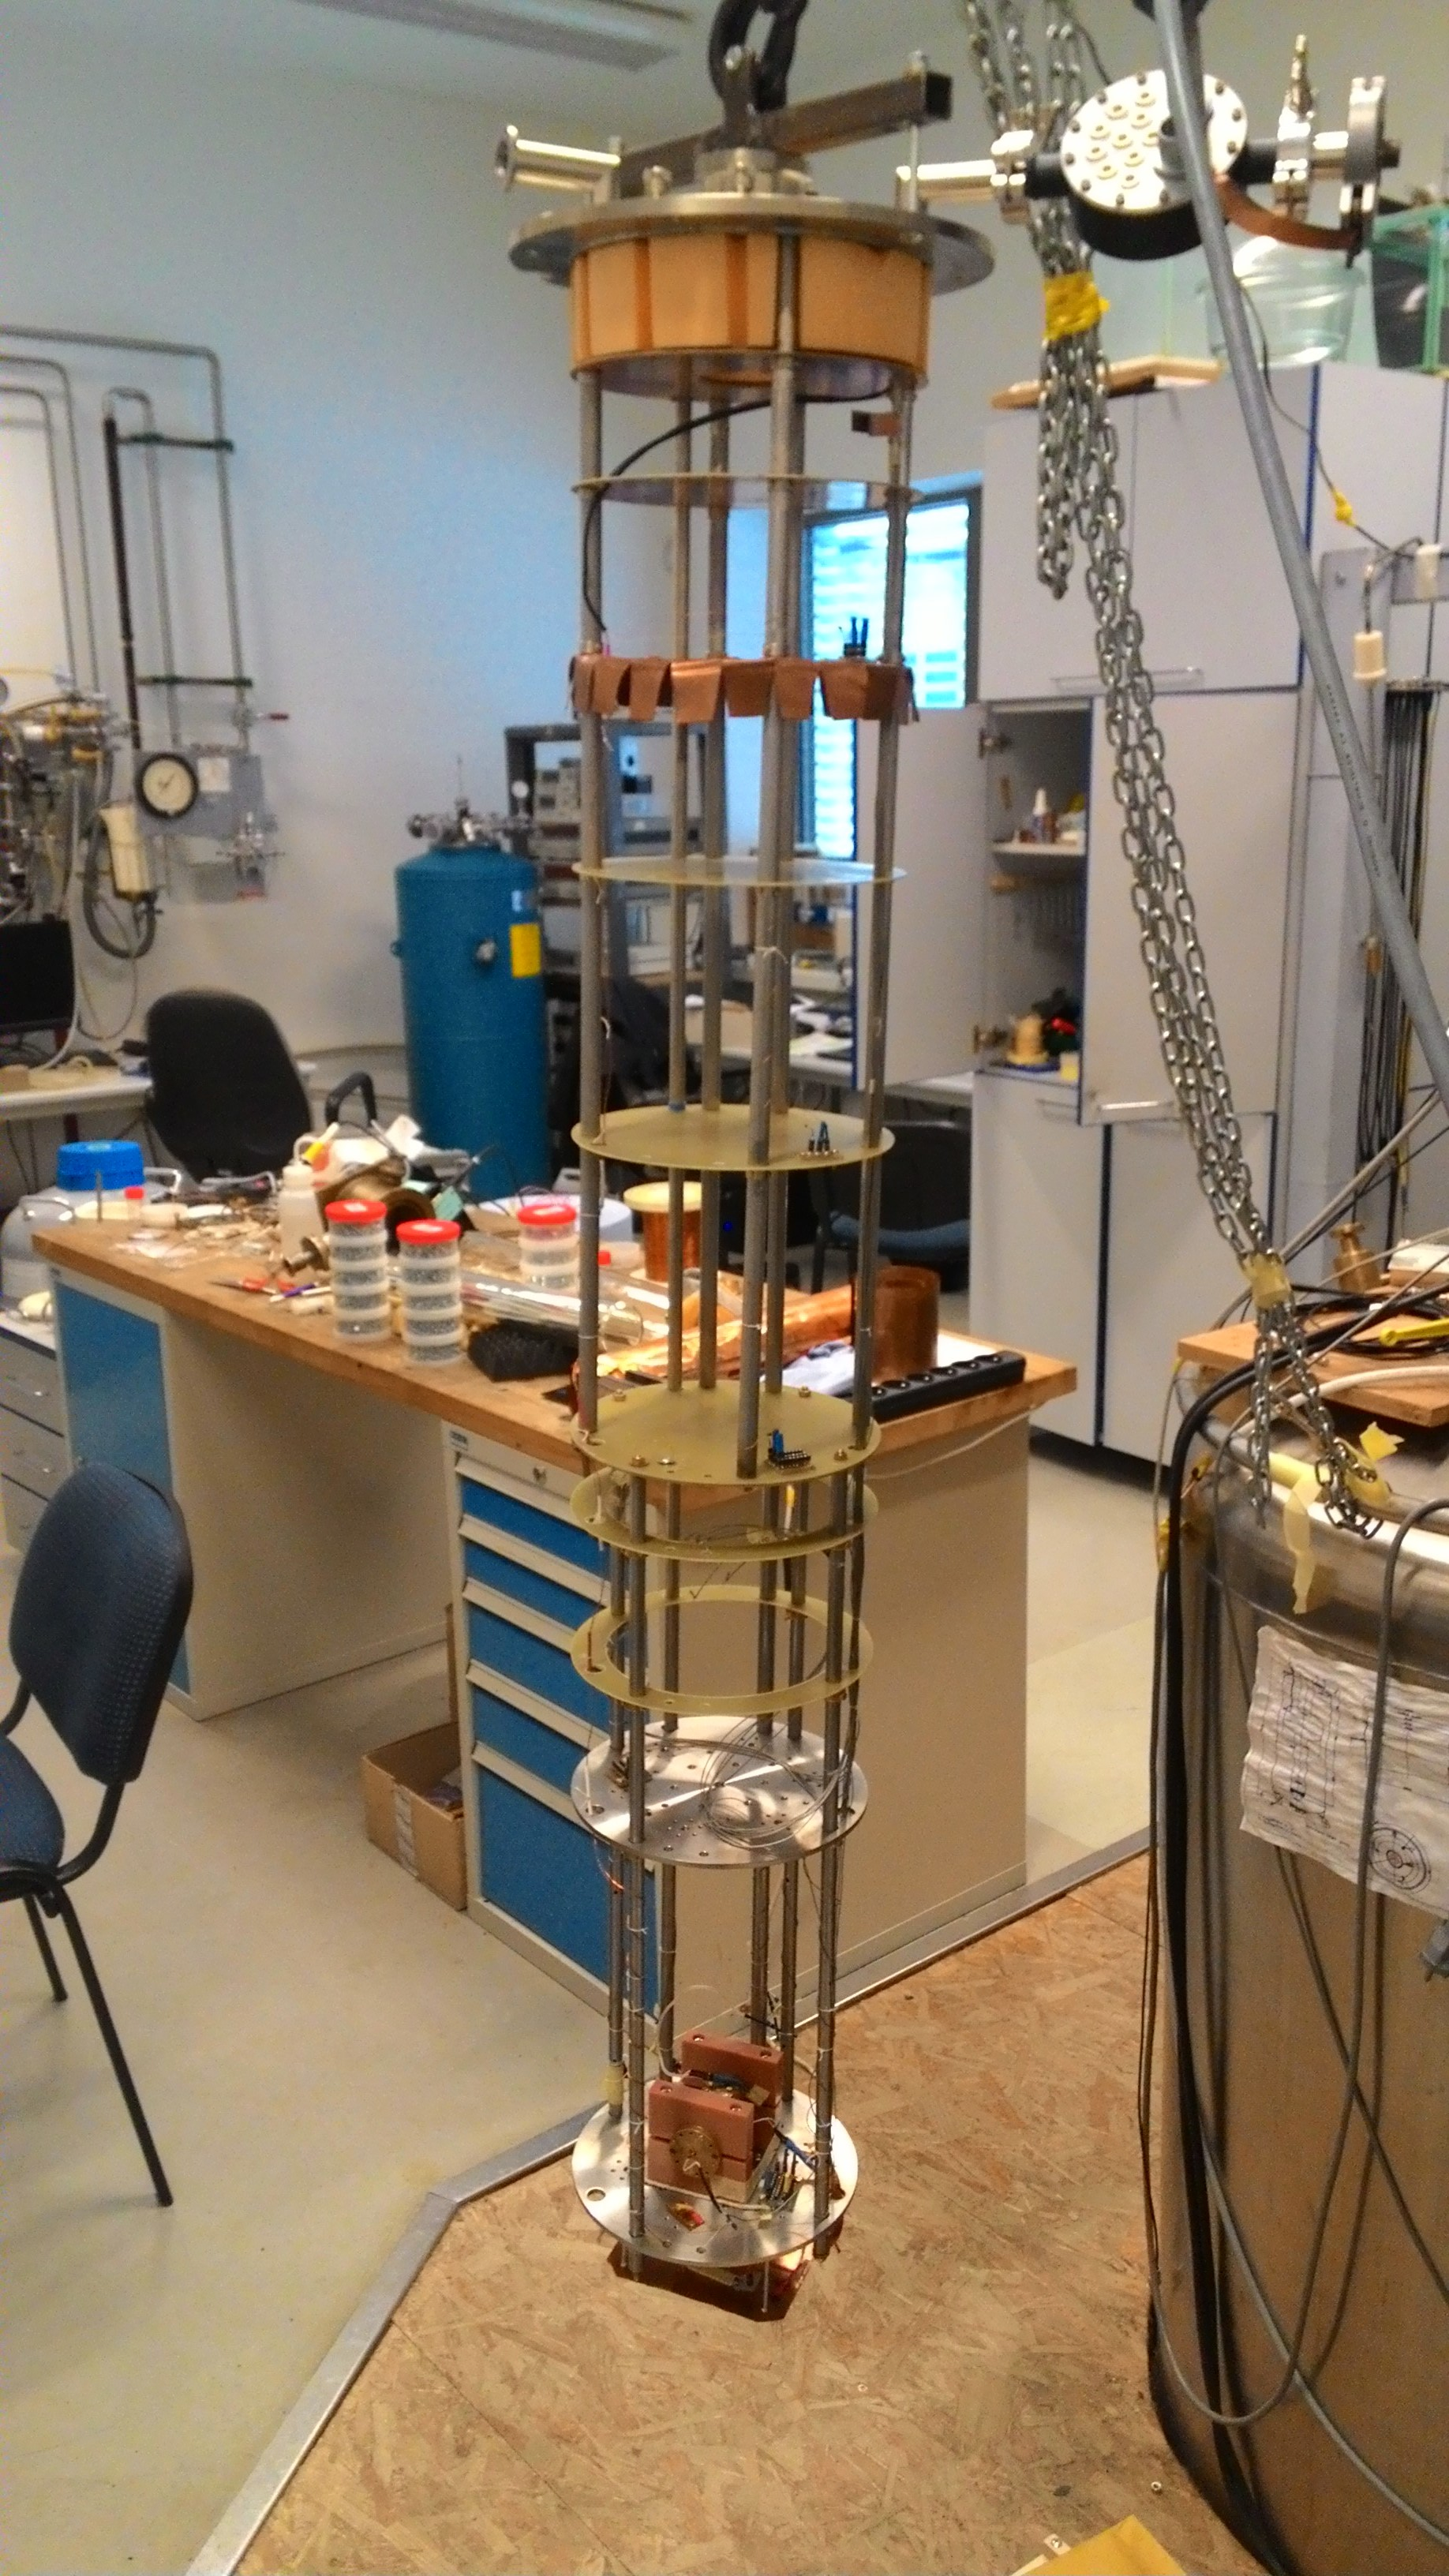
\includegraphics[width=0.5\textwidth]{graphics/exp/insert}
	\caption{abcd}
\end{figure}

Chamber:

\begin{figure}[h]
	\centering
	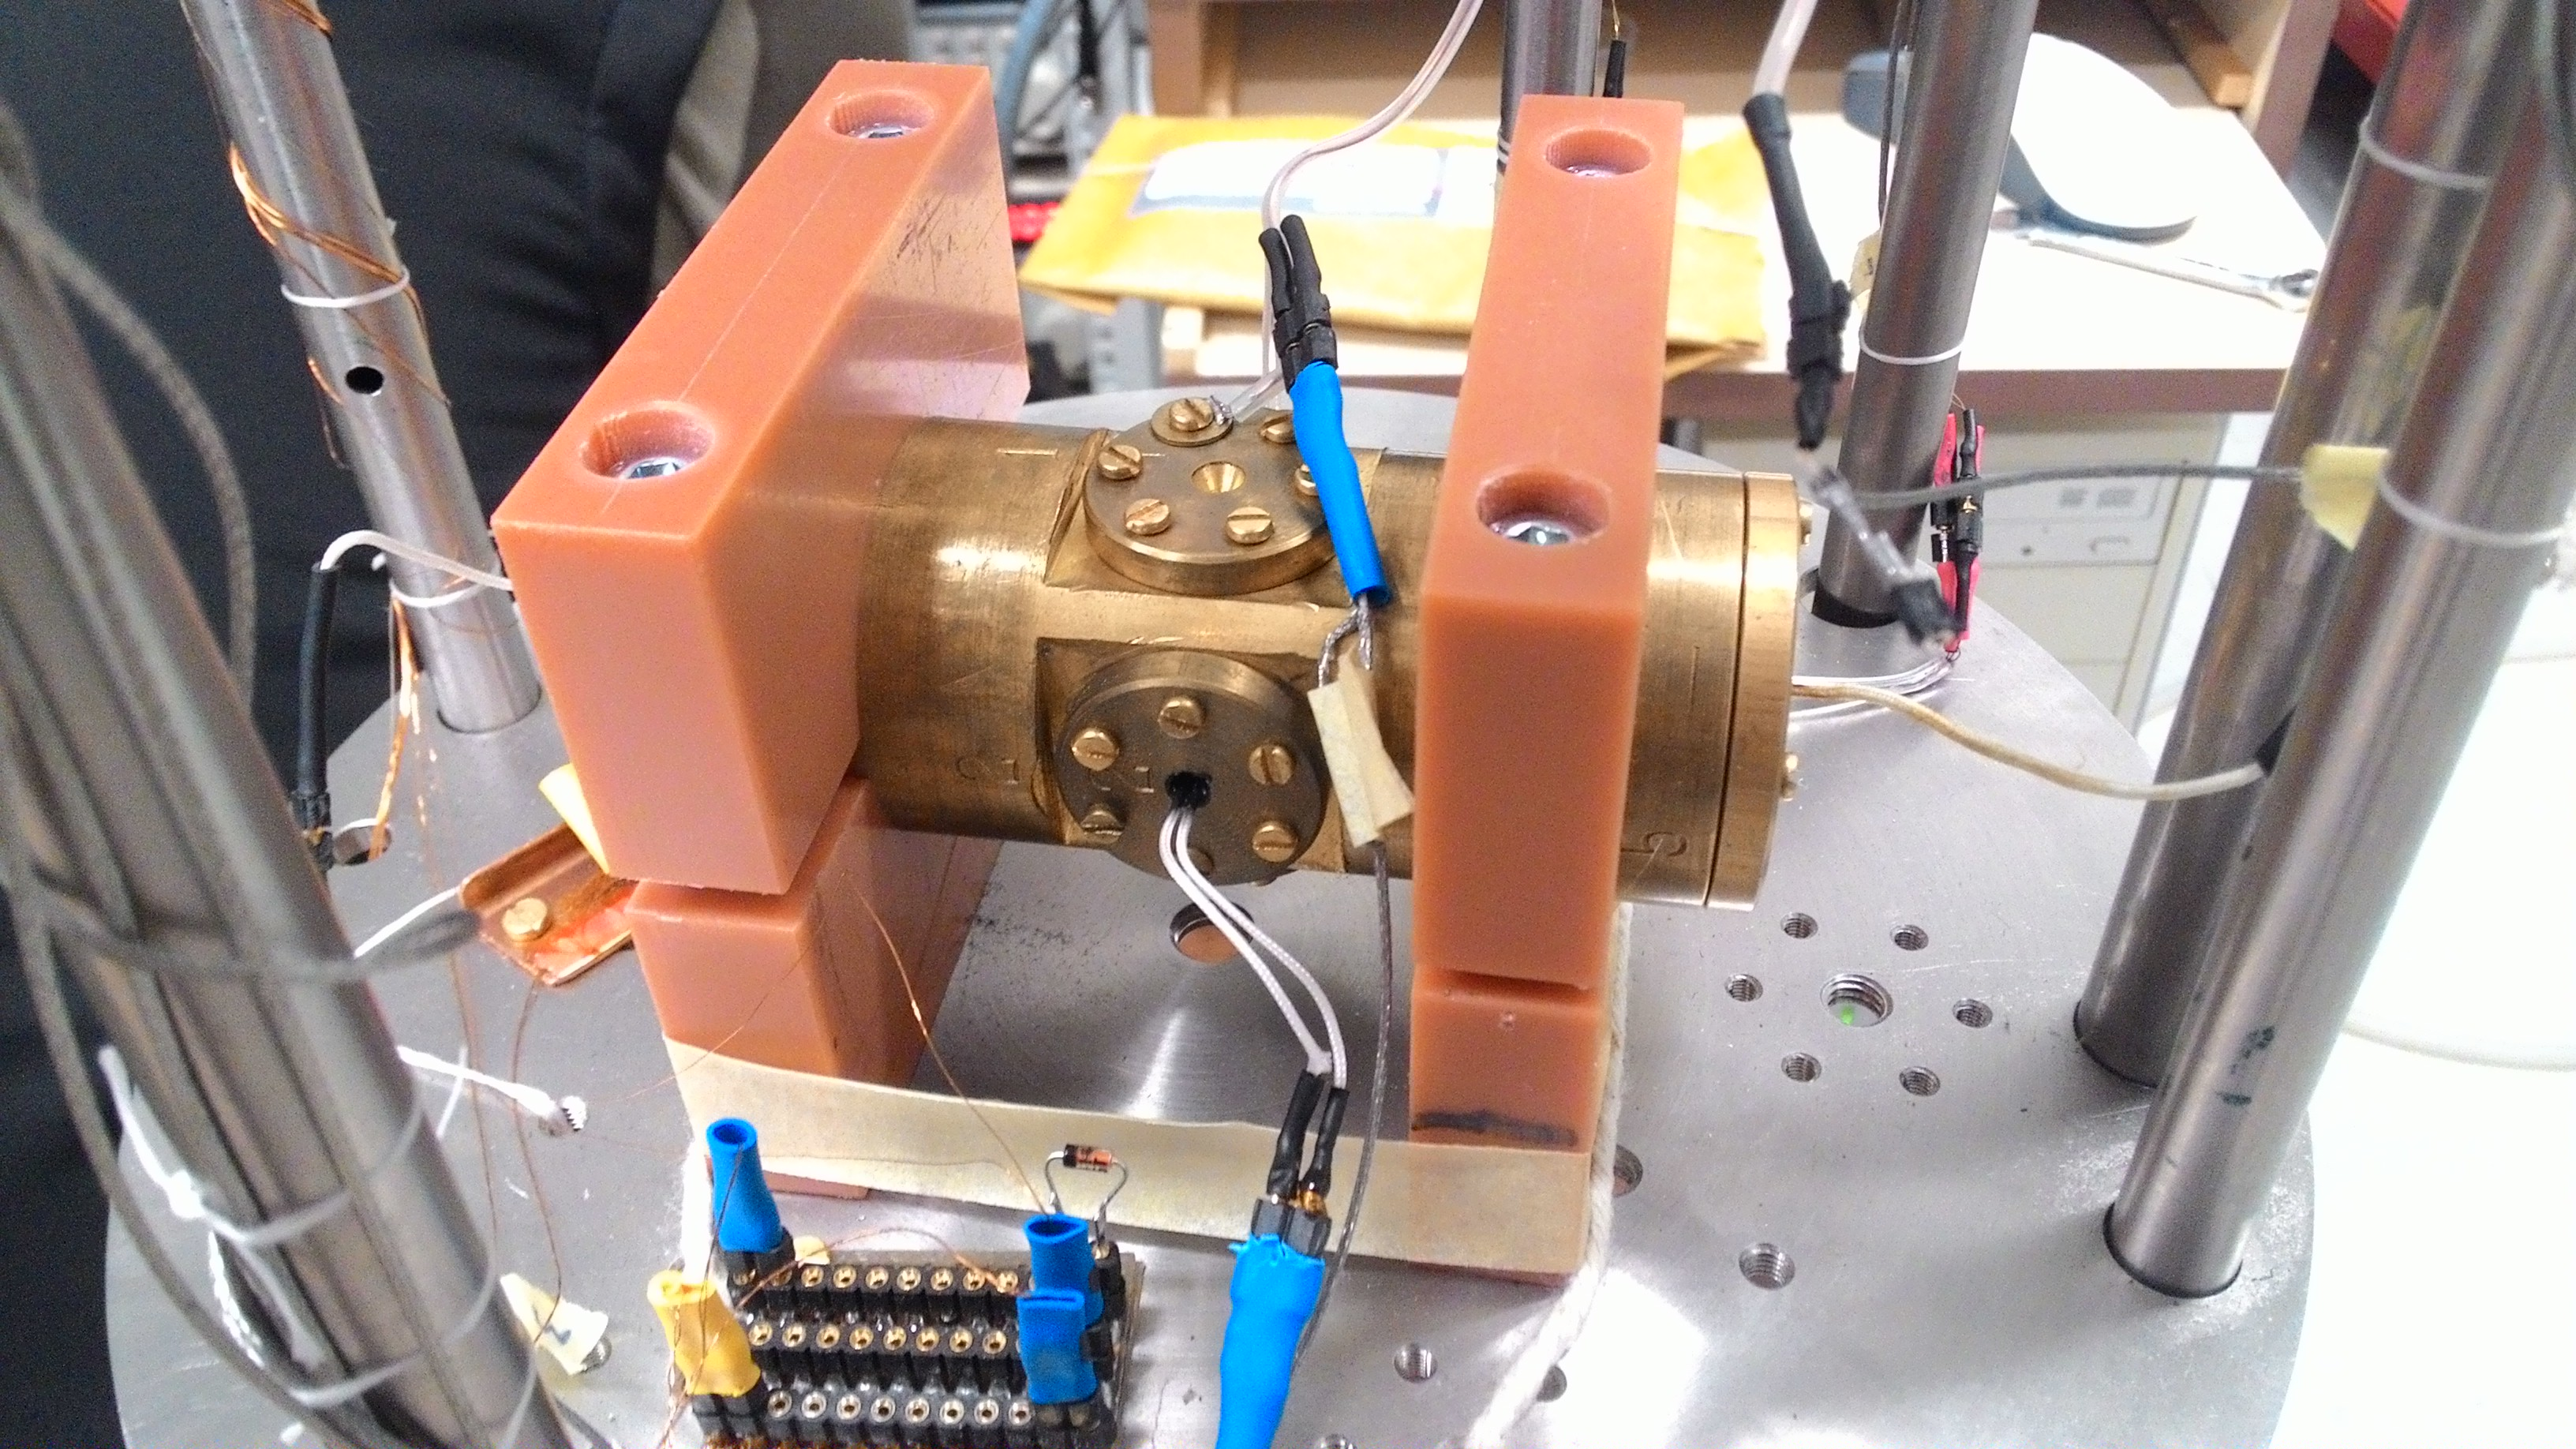
\includegraphics[width=0.5\textwidth]{graphics/exp/chamber}
	\caption{abcd}
\end{figure}

\section{Generation of QT}

From the variety of oscillating candidates we chose the most available and reliable one - the quartz tuning fork. Quartz tuning forks (TF) are commercial piezoelectric oscillators with a well-calibrated resonant frequency. They are usually used as frequency standards in watches or as force sensors in microscopes. Also, TFs have started to be widely used in cryogenic Helium II experiments.

In this work, we used the fork of following dimensions: prongs length $ \mathcal{L} = 3.50\unit{mm} $, prongs width (perpendicular to the fork plane) $ \mathcal{W}=75 \mu\unit{m} $, thickness $ \mathcal{T}=90\mu\text{m} $ prongs interdistance $ \mathcal{D}=90\mu\text{m} $. A sketch of the fork architecture is depicted below:

\begin{figure}[h]
	\centering
	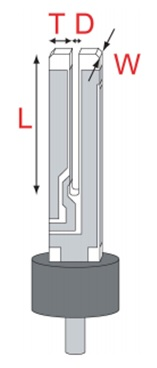
\includegraphics[width=0.25\textwidth]{graphics/exp/quartz}
	\caption{Labeled depiction of the tuning forks}
\end{figure}

There are several achievable resonant modes at which the fork can oscillate. We chose to work with the \textit{fundamental} one at $f_0 = 6.5 \unit{kHz}$ and with the first \textit{overtone} one at $f_1 = 40 \unit{kHz}$.\\
The fork is driven by applying an alternate voltage $V(t) \propto e^{i\omega t}$ from a generator to the metalic plates (deposited on fork surface). The piezoelectric effect causes a tension resulting in a force, which is proportional to the applied voltage. In fundamental mode, the fork exhibits an anti-phase oscillating motion of its prongs with a single node. In case of overtone, there would be just two nodes. The fork's flex induces a piezoelectric current $I(t)$ about which is shown its proportionality to the velocity $U(t)$.

The conversion relations between applied $V(t)$, resulting $I(t)$ and mechanical properties $F(t)$, $U(t)$ are:

\begin{equation}
F(t) = \frac{1}{2} a_{rmf} V(t)\,,
\hspace{1cm}
U(t) = \frac{I(t)}{a_{rmf}}\,,
\end{equation}

where $a_{rmf}$ is the so-called \textit{fork constant}. This constant can be derived from a fork's geometry, material and an oscillation mode. Usually the formula for this constant is given by a deflection measurement:

\begin{equation}
a_{rmf} = \sqrt{4\pi m_{eff} \Delta f \frac{I}{V}}\,,
\end{equation}

where $m_{eff}$ id the fork's effective mass and $\Delta f$ is the measured peak width from the fequency-sweep deflection measurement. In case of our used fork, the effective mass and fork constants for fundamental and overtone modes, respectively:

\begin{equation}
m_{eff} = 1.52 \times 10^{-2} \mu\unit{g}\,,
\hspace{1cm}
a_0 = 0.36 \mu\unit{Cm}^{-1}\,,
\hspace{1cm}
a_1 = 1.38 \mu\unit{Cm}^{-1}
\end{equation}

\subsection*{Other resonators}
\todo

\section{QT Detection}
\begin{itemize}
	\item Second sound generating
	\item SS detection
\end{itemize}

SS sensor:

\begin{figure}[h]
	\centering
	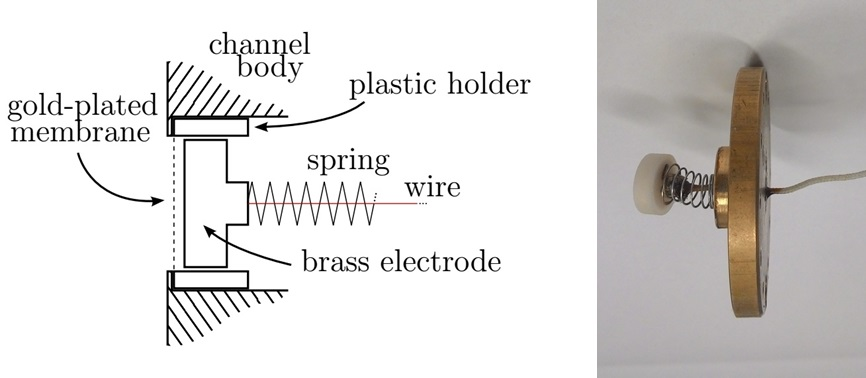
\includegraphics[width=0.8\textwidth]{graphics/exp/sensor}
	\caption{abcd}
\end{figure}

Resonator scheme:

\begin{figure}[h]
	\centering
	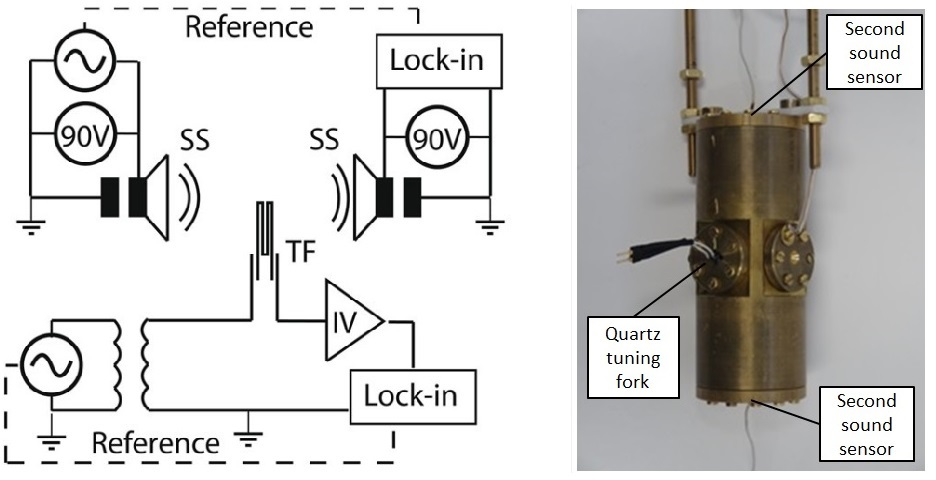
\includegraphics[width=0.8\textwidth]{graphics/exp/resonator}
	\caption{abcd}
\end{figure}


\section{Measurement methods and Processing}
\begin{itemize}
	\item fork modes - fund, overtone
	\item SS modes - working with ??-th mode
	\item frequency sweeps
	\item amp sweeps
	\item constant drives with SS on/off
\end{itemize}

As an observational technique we used the attenuation of second sound, which also serves to mesure the length of vortex line per unite volume $L$ in superfluid component.

It was shown that a pure classical model could explain the observed time decay of line length $L$. According to this model, superfluid Helium II behaves as a single fluid with a scaled
kinematic viscosity $\mu^{\prime}$. After an initial time interval, the turbulent energy spectrum has the classical Kolmogorov form $E(k) \propto \eps^{2/3} k^{-5/3}$ and thus energy is continually transferred in a cascade from lower to higher wave numbers. In finite container, the
classical theory predicts the time decay of vortex lin density $L$ as:

\begin{equation}
L(t) \propto \frac{(3C_D)^{3/2}}{\sqrt{\mu^{\prime}}} t^{-3/2}
\end{equation}

\newpage
